\chapter{Теоретический базис} \label{chapt1}

Распространение функции взаимной когерентности~\ref{eq:g1} поля $E(r, \omega)$ через свободное пространство от некогерентных стационарных источников излучения описывается теоремой Ван Циттера - Цирнике \cite{van_cittert_wahrscheinliche_1934}, \cite{zernike_concept_1938}. 
\begin{align}
	g^{(1)} (r_1; r_2) = \cfrac{\big \langle \bar{E}(r_1) \bar{E}(r_2) \big \rangle}{\big \langle \bar{E}(r_1)\big \rangle \big \langle\bar{E}(r_2) \big \rangle}, 
	\label{eq:g1} 
\end{align}
где $\big \langle ... \big \rangle$ означает усреднение по статистическим реализациям поля. Теорема даёт связь между распределением интенсивности источника излучения $I(\xi, \eta)$ и функцией взаимной когерентности $g^{(1)} (r_1, r_2)$ через двумерное Фурье преобразование. 
\begin{align}
	g^{(1)} (x_1, y_1, x_2, y_2) = \cfrac{\kappa e^{-i\psi}}{(\bar{\lambda}z)^2} \iint \limits_{-\infty}^{+\infty} I(\xi, \eta) \exp{\big [(i \cfrac{2 \pi}{\bar{\lambda}z}) (\Delta x \xi + \Delta y \eta)\big]}d\xi d\eta, 
	\label{eq:van_cittert_zernike_theorem} 
\end{align}
где $\kappa = \bar{\lambda}^2 / \pi$, $\bar{\lambda}$ -- средняя длина волны квазимонохроматического источника излучения, $z$ -- расстояние до плоскости наблюдения от источника излучения, $\psi = \cfrac{\pi}{\bar{\lambda} z}\big[((x^2_2 + y^2_2) - (x^2_1 + y^2_1)) \big]$, а $\Delta x = x_2 - x_1$, $\Delta y = y_2 - y_1$

\begin{figure}[H] 
	\centering 	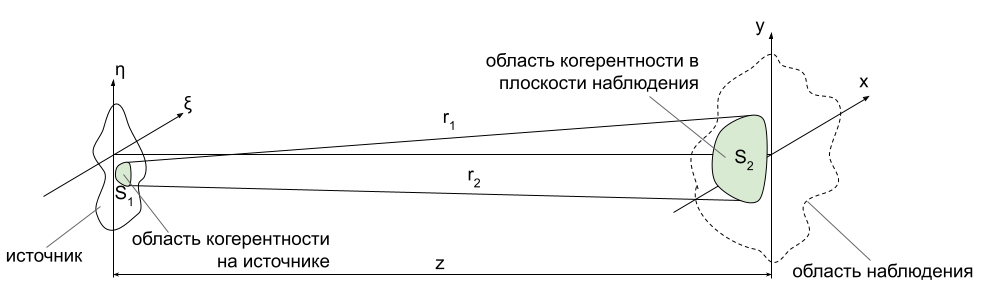
\includegraphics[width=0.99\linewidth]{VCC_scheme.png}
	\caption{К формулировке теоремы Ван Циттерта-Цернике}
	\label{fig:VCC_scheme}
\end{figure}

Теорема может быть видоизменена и сформулирована для частично когерентных источников излучения достаточно лишь заменить $\kappa$ на двойной интеграл \cite{goodman_statistical_2015}
\begin{align}
	\kappa(\bar{x}, \bar{y}) = \iint \limits_{-\infty}^{+\infty} \mu(\Delta \xi, \Delta \eta) \exp{\big [(i \cfrac{2 \pi}{\bar{\lambda}z}) ( \bar{x} \Delta \xi + \bar{y} \Delta \eta)\big]}d\Delta \xi d\Delta \eta, 
\end{align}
где $\bar{x} = \cfrac{x_1 + x_2}{2}, \bar{y} = \cfrac{y_1 + y_2}{2}$,  $\Delta \xi = \xi_2 - \xi_1$, $\Delta \eta = \eta_2 - \eta_1$. Таким образом, следую модифицированной теореме ван Циттер-Цирнике, область пятна когерентности на расстоянии $z$ будет определяться не только размером источника излучения, но и размером области когерентности на самом источнике. 

В качестве примера распространения когерентности от полностью некогерентного источника можно оценить область когерентности излучения лабораторной рентгеновской трубки. Область когерентности от полностью некогерентного источника излучения квадратной формы получается напрямую из теоремы ван Циттер-Цирнике
\begin{align}
	A_c = \cfrac{(\bar{\lambda} z)^2}{A_s}.
\end{align}
Подставляя $z = 1$ м и $\lambda \approx 0.7$ $\textup{\AA}$ со спроецированной на направление выхода излучения из рентгеновской трубки площадью фокального пятна меньше чем $A_s = 1$ $\textup{мм}^2$ \cite{cullity_elements_1956}. Таким образом линейный размер длины когерентности при отражении от исследуемого кристалла с учётом угла дифракции ($\sim 45^{\circ}$) будет порядка $0.1$ $\textup{мкм}$. Однако линейный размер пятна когерентности может быть увеличен до нескольких микрон при использовании трубки с вращающимся анодом, где характерный диаметр круглого источника достигает $50$ $\textup{мкм}$ \cite{cullity_elements_1956}.  

Для синхротронных источников излучения область когерентности на источнике определяется натуральным размером излучения одного электрона при пролёте через вставное устройство. Например, в случае ондуляторного источника натуральный размер излучения определяется геометрическим размером перетяжки излучения в центре ондулятора. В случае рассмотрения излучения целого электронного пучка необходимо сравнивать размер излучения в перетяжке с размером электронного пучка. Для точного описания излучения от всего электронного пучка электромагнитное излучение может быть представлено как сумма полей от каждого индивидуального электрона. Каждый $k$ электрон в пучке имеет свою координату -- $\vec{\eta}_k$, угол -- $\vec{\l}_k$, отсчитываемые от проектной траектории, а также продольную координату или, другими словами, время прибытия $t_k$ относительно некоторого времени $t_0$, вклад которого в $r\omega$-пространстве будет умножением поля на фазовый фактор $\exp{(i \omega t_k)}$. Указанные величины подчиняются некоторым распределениям плотности вероятности, для накопительных колец в модельных случаях это распределение Гаусса. В данном случае не рассматривается разброс электронов по энергии, а дальнейшие описание можно найти в \cite{geloni_effects_2018}. Объём фазового пространства, который составляют эти шесть переменных, и есть эмиттанс электронного пучка. Результирующее поле от $N_e$ электронов можно записать следующим образом:
\begin{align}
	\bar{E}_{b} (z, \vec{r}, \omega) = \sum\limits_{k=1}^{N_e} \bar{E}(\vec{\eta}_k, \vec{\l}_k, z, \vec{r}, \omega) \exp{(i \omega t_k)},
	\label{eq:E_bunch} 
\end{align}
Для электронов в накопительных кольцах случайные величины $\vec{\eta}_k$ и $\vec{\l}_k$ не зависят от времени прибытия $t_k$. Модуля поля $\bar{E} = |\bar{E}_k|\exp{i\phi_k}$ имеет независящей от $k$ одинаковое распределение со средним $\big \langle|\bar{E}_k|\big \rangle$ и конечным вторым моментом  $\big \langle|\bar{E}_k|^2\big \rangle$. \rr{Всё это здорово, но должно откуда-то следовать. По всей видимости, эти предположения следуют из наличия дробового шума в электронном пучке (затухание и квантовая раскачка бетатронных колебаний). Нужна объяснительная команда.}.

Результирующее поле $\bar{E}_{b}$ является суммой вкладов от каждого электрона в пучке и по своей структуре в правой части уравнения~\ref{eq:E_bunch} записан некоторый фазор. Следуя предпосылкам центральной предельной теоремы (ЦПТ), можно показать, что $\bar{E}_{b}$ комплексная Гауссова переменная. Другими словами, амплитуда поля в каждой точке $\vec{r}$ подчиняется гауссовому распределению. Однако, предпосылки ЦПТ выполняются для двух практически значимых предельных случаев: случай длинного $\omega\sigma_T \gg 1$ и короткого электронного пучка $\omega\sigma_T \gg 1$, где $\sigma_T$ -- длительность электронного пучка \rr{а что не так с $\omega\sigma_T \sim 1$?}. В случае длинного электронного пучка величина $\omega t_k$ равномерно распределена в пределах от $0$ до $2\pi$ и излучение продольно некогерентно, для короткого пучка фазовый множитель $\exp{(i \omega t_k)}$ может быть взят равным единице и излучения является продольно когерентным. 

\rr{тут необходимо вернуться к идее о размер излучения одного электронна и размере электронного пучка}
\rr{так же где-то упомянуть о продольной спайковой структуре}
\newpage
%============================================================================================================================






